
Attack graphs have long been modeled as probabilistic processes\cite{ Dacier_Deswarte_Kaaniche, Ortalo_1999, Phillips_Swiler_1998, Weiss_1991}. We consider the movement of an attacker through the nodes of the attack graph as a stochastic process and interpret the state of the system as the current position of the attacker in our network. An attacker can advance to another state in the process through successful compromise of the vulnerability represented by that state only if there exists an edge in the attack graph between the attacker’s current state and the advance state.  The collection of all states in the process is the system’s state space and corresponds to the set of nodes in our attack graph. Advancing to another state is probabilistic and the success of the advance is based on the weighted score associated with that node. For example, from Figure \ref{fig:tg_001}, if the attacker is at Node 3, the probability that the target will be compromised is only based on the difficulty of exploiting the vulnerability on Node 1 (Trojan installation), and not on the path the attacker took to arrive at Node 3.

Because we only need to rely on the current state of the system and not how the system arrived in that state to determine the next state, we are able to model the attack graph as a Markov Chain without loss of generality. A Markov Chain is a stochastic process that is \textit{stateless}, that is, prediction of the next system state can be made based only on the current state. This is known as the Markov Property.  

More formally, for a stochastic process \(X = {X_t, t \geq 0}\), if the attack graph has \(n\) nodes, then the set of possible states, \(S\), for \(X\) is \(S = {s_1, s_2, \ldots, s_a, \ldots, s_n}\). The probability \(P_i,j\) that an attacker in state \(X_t\) will advance to state \(X_{t+1}\) can be given as \(P(X_{t+1} = j | X_t = i)\) with the Markov Property being satisfied as: 
\[P(X_{t+1} = j | X_1 = x_1 , X_2 = x_2 , \ldots, X_t = i)  = P(X_{t+1} = j | X_t = i) \]
The value \( P_{i,j}\) is known as the transition probability between two states\( s_i\) and \(s_j\). We can model the n states of the process \(X\) as an \(nxn\) matrix whose\( (i, j) \)entry is the transition probability\( P_{i,j}\).

The transition matrix
\[
P = \begin{bmatrix} 
    P_{11} & \dots & P_{1n}  \\
    \vdots & \ddots & \\
    P_{n1} &        & P_{nn} 
    \end{bmatrix}
\]
must also satisfy the conditions:  

\[0 \leq P_{i,j} \leq 1\quad for\quad i,j \in S\]

\[\sum_{j=1}^{n} P_{i,j} = 1\]

That is, if a state has three outbound edges (possible choices to exploit next), the probability that any edge is followed is \(1\) since we must proceed to the attack goal after each time step, and the probability a specific edge is followed is determined by how exploitable that vulnerability is (the transition probability). This stochastic model enables us to study the system’s quantitative and qualitative properties through well-established analytic and simulation methods. Assuming the system state is given as the attacker’s current location on the attack graph (the vulnerability most recently exploited), we can model the system’s subsequent states through iteration of the stochastic process over discrete time intervals.  

 

Attack graphs in general have the special property that the attack goal can be reached from any node in the network, allowing us to model them as an Absorbing Markov Chain using the transition matrix described above. An Absorbing Markov Chain is a Markov Chain that includes at least one absorbing state, in our case the attack goal. The absorbing state can be reached from all other states, and once the absorbing state is reached (the attacker has compromised the target), no further transitions are considered.  

\begin{figure}[ht]
\centering
\includegraphics[width=.8\textwidth]{resource/img/ch_background/sdn_analytics/eg_trans_diagram.png}
%%\includegraphics[width=100mm]{content/figs/eg_trans_diagram.png}
\caption{Example Transition Diagram}
\label{fig:ag_2}
\end{figure} 

In Figure \ref{fig:ag_2} we see a  notional transition diagram. The possible states in the chain are connected by edges labeled with the probability of advancing to an adjacent state (successfully exploiting the next vulnerability.) The self-referencing edges represent the probability of an unsuccessful exploit and occur at entries \(Pi,i\) along the diagonal of the transition matrix. Note that once the system enters the ‘Target’ state no other state is reachable which we define as the absorbing state.  

 

To create a transition matrix that conforms to the definition of an absorbing Markov chain, each outbound edge is assigned a transition probability calculated by normalizing the CVSS exploitability scores associated with all adjacent (next-step) states. That is, if we are at state \(S_i \)and the set of possible next states are given as \(S_{i+1} = {s1, s2, \ldots, sn}\) then we calculate the transition probability
\[ Pij =\frac{CVSS(s_j)}{\sum_{k=1}^{n}CVSS(s_k)}; k \in S_{i+1}\]
This normalizes the transition probabilities for all outbound states of a given node and guarantees the two conditions for a Markov transition matrix defined above will be satisfied.  

 

The transition matrix \( P\) for the absorbing Markov chain defined above can be put into the canonical form \( P=\)
\(\begin{bmatrix}
Q & R \\
0 & I
\end{bmatrix}\)
  where \(Q\) is the matrix of transition probabilities for moving from a non-absorbing (transient) state to another transient state, and \(R\) is the matrix of transition probabilities for moving from a transient state to an absorbing state. In other words, we can order the rows and columns such that all transient states precede the absorbing states.  

 

From the canonical form, \(P_k\) approaches some limiting matrix \(|P|\) as \(k\) increases, where\( |P|=\)
\(\begin{bmatrix}
0 & FR \\
0 & I
\end{bmatrix}\)
  and \(F = (I-Q)-1\). This matrix \(F\) is known as the fundamental matrix for \(P\), and it allows us to derive many interesting properties from our system. For example, the\( (i, j)\) entries of \(|P|\) provide the long-term (limiting) probabilities of advancing from state \(i\) to state \(j\). Likewise, the sum of the row  entries in \(F\) determine the average number of steps it will take to reach an absorbing state from each transient state. 

Note that for the transition matrix \(P\) defined above, the entry \(P_{i, j}\) is the probability the system given initial state \(s_i\) will move to state \(s_j\) on the next step. It follows from the total probability theorem that the probability the system will be in state \(s_j\) after exactly two time steps is the \((i, j)\) entry of:  
\[
P^2=
\begin{bmatrix}
Q & R \\
0 & 1
\end{bmatrix}
\begin{bmatrix}
Q & R \\
0 & 1
\end{bmatrix}=
\begin{bmatrix}
Q^2 & QR + R \\
0 & 1
\end{bmatrix}
\]
After 3 time steps:
\[
P^3=
\begin{bmatrix}
Q^2 & QR + R \\
0 & 1
\end{bmatrix}
\begin{bmatrix}
Q & R \\
0 & 1
\end{bmatrix}=
\begin{bmatrix}
Q^3 & Q^2R +QR + R \\
0 & 1
\end{bmatrix}
\]

 
 …, and after t time steps: 
 \[
P^t=
\begin{bmatrix}
Q^t & (I + Q +Q^2 ... +Q^{t-1}) R \\
0 & 1
\end{bmatrix}
\]
 We have defined \(Q\) as the matrix of transient probabilities with values less than \(1\), so it holds that \(Q^t \to 0\) as \(t \to \infty\)
(eventually we will reach the attack target). Now consider the matrix  \(F\) such that \( F= I + Q + Q^2 +...\)

The values of \(Q^t(i,j)\)  then are the probabilities of the system starting in state \(s_i\) and ending in state \(s_j\) exactly \(t\) steps later. In this case we can interpret the probability \(Q^t(i,j)\)
  as the fraction of time period \(t\) spent in state \(s_j\), so the total number of periods the process occupies state \(s_j\) before becoming absorbed is:  \(F(i, j) = Q^0(i,j)+Q^1(i,j)+Q^2(i,j)...\) and the reduced form is known as the \textbf{fundamental matrix:}
\[ F = (I-Q)-1\] 


% we have scripted the process of parsing the MulVal output, reducing and coalescing the nodes into a format compatible with the Cyber Security Analytics Framework, performing the lookup of CVSS scores for known vulnerabilities, and calculating the transition probabilities. 

% *The transition matrix provides a key input for stochastic modeling, which will be used to produce the final metrics through simulation or analytical means. 

% *Finally, the attack graph encoded with the desired transition probabilities is used as input for the metric derivation model, in this case using Markov chains. The model is run under simulation or solved analytically to produce the desired metric output suitable for comparison.  

%  The result is the fundamental matrix used as input to stochastic models to calculate the various metrics.  


% Section \ref{sec_contributions} details the design and implementation with a supporting case study in section \ref{sec_approach}. 

\textbf{Node Ranking (NR):  }

We have shown that the elements of the fundamental matrix \(F\) take on values that represent the relative duration of time spent at each transient node in the Markov process. In the context of our security analysis, these values equate to the amount of hold time we expect an attacker to incur while trying to advance to the target. Lower node rankings indicate nodes along the attack path that are relatively easy for an attacker to clear. If a difficult to exploit vulnerability exists and its associated NR is relatively low this might be an indication that a security control point is being bypassed. Using the attack graph and associated NR analysis it is a fairly straight forward process to identify the area of interest and trace back to the origin of the bypass. Liu\cite{Liu_Singhal_Wijesekera} examines this process of forensic reconstruction of attacks using attack graphs in detail.

\textbf{Probabilistic Path (PP):} 

The PP metric is another interesting property derived from our Markov transition matrix. Taking the product of the fundamental matrix F and the matrix of absorbing probabilities \(R\) results in a matrix, \(B = FR\), whose \(B(i,j) \) entries yield the probability of being absorbed by state \(s_j\) given we started at initial state \(s_i\).  

\textbf{Expected Path Length (EPL):  }

We define EPL as the expected number of time steps required for an attacker to advance from the initial state to the attack goal, and its calculation follows as a direct consequence of deriving the NR metric. That is, if the NR metric expresses the total expected time that a process starting in initial state $s_i$ will occur in transient state \(s_j\) before ultimately being absorbed, then the NR sum over all transient states for \(s_i\) will predict the total time spent in the process before absorption. To take the sum of the values in the rows of the fundamental matrix we multiply by a column of 1’s, $t = N1$, and the entry \(t_i\) contains the EPL value for initial state \(s_i\). 
 

\textbf{Mean Time To Failure (MTTF)} 
Time based metrics are a subset of probabilistic measures used to estimate how long it will take for some target objective to be met\cite{Dacier_Deswarte_Kaaniche}\cite{Ortalo_1999}\cite{McQueen_Boyer_Flynn_Beitel_2005}. 

% MTTF is the measure of the mean time for an attacker to reach a target. This measure directly maps to Expected Path Length as we have defined it. 

% \textbf{Mean Time To Failure (MTTF)} 

% MTTF is the measure of the mean time for an attacker to reach a target. This measure directly maps to Expected Path Length as we have defined it above. 

% \textbf{Mean Time To Breach (MTTB)} 

% MTTB is the measure of the mean time for an attacker to reach a target. 

% \textbf{Mean Time To Failure (MTTR)} 

% MTTR is the measure of the mean time for an attacker to reach a target. 